\documentclass[border=3pt]{standalone}
\usepackage{fontspec}
\setmainfont{Times New Roman}
\usepackage{pgfplots}
\pgfplotsset{compat=1.18}
\usetikzlibrary{arrows.meta,calc,positioning,shapes.geometric}
\definecolor{forest}{HTML}{346E57}
\definecolor{sage}{HTML}{E8EFEA}
\definecolor{clay}{HTML}{B77E60}
\definecolor{gray}{HTML}{718078}
\definecolor{rule}{HTML}{B7C3BA}
\definecolor{ink}{HTML}{000000}
\begin{document}
\hyphenpenalty=10000\exhyphenpenalty=10000
\fontsize{10}{12}\selectfont
\renewcommand{\small}{\fontsize{9}{11}\selectfont}
\renewcommand{\scriptsize}{\fontsize{8}{10}\selectfont}
\resizebox{16cm}{!}{%
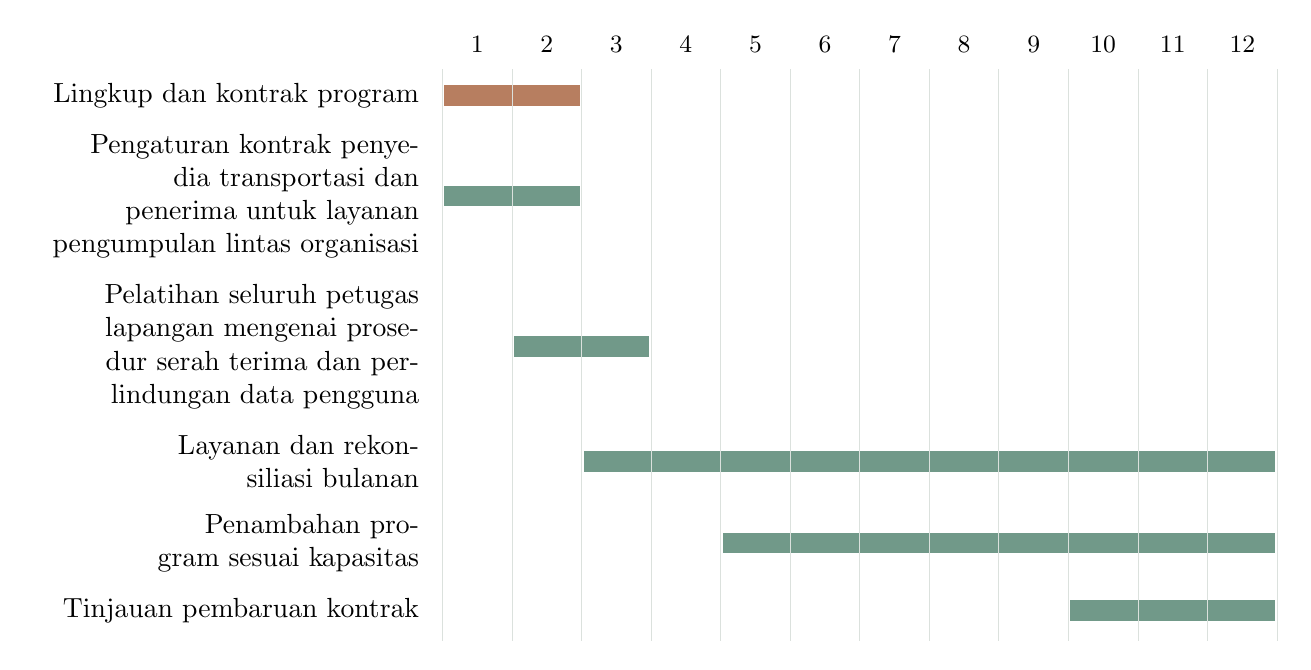
\begin{tikzpicture}[x=1cm,y=1cm]
\node[anchor=north east,text width=4.9cm,align=right,inner sep=2pt] (task0) at (-.22,0) {Lingkup dan kontrak program};
\coordinate (row0) at (0,0 |- task0.center);
\fill[clay] ($(row0)+(0.025,-.13)$) rectangle ($(row0)+(1.7416666666666667,.13)$);
\node[anchor=north east,text width=4.9cm,align=right,inner sep=2pt] (task1) at ($(task0.south east)+(0,-.18)$) {Pengaturan kontrak penyedia transportasi dan penerima untuk layanan pengumpulan lintas organisasi};
\coordinate (row1) at (0,0 |- task1.center);
\fill[forest!70] ($(row1)+(0.025,-.13)$) rectangle ($(row1)+(1.7416666666666667,.13)$);
\node[anchor=north east,text width=4.9cm,align=right,inner sep=2pt] (task2) at ($(task1.south east)+(0,-.18)$) {Pelatihan seluruh petugas lapangan mengenai prosedur serah terima dan perlindungan data pengguna};
\coordinate (row2) at (0,0 |- task2.center);
\fill[forest!70] ($(row2)+(0.9083333333333333,-.13)$) rectangle ($(row2)+(2.625,.13)$);
\node[anchor=north east,text width=4.9cm,align=right,inner sep=2pt] (task3) at ($(task2.south east)+(0,-.18)$) {Layanan dan rekonsiliasi bulanan};
\coordinate (row3) at (0,0 |- task3.center);
\fill[forest!70] ($(row3)+(1.7916666666666665,-.13)$) rectangle ($(row3)+(10.575,.13)$);
\node[anchor=north east,text width=4.9cm,align=right,inner sep=2pt] (task4) at ($(task3.south east)+(0,-.18)$) {Penambahan program sesuai kapasitas};
\coordinate (row4) at (0,0 |- task4.center);
\fill[forest!70] ($(row4)+(3.558333333333333,-.13)$) rectangle ($(row4)+(10.575,.13)$);
\node[anchor=north east,text width=4.9cm,align=right,inner sep=2pt] (task5) at ($(task4.south east)+(0,-.18)$) {Tinjauan pembaruan kontrak};
\coordinate (row5) at (0,0 |- task5.center);
\fill[forest!70] ($(row5)+(7.975,-.13)$) rectangle ($(row5)+(10.575,.13)$);
\coordinate (gridBottom) at ($(task5.south)+(0,-.16)$);
\node[font=\small,text width=0.8033333333333333cm,align=center,anchor=south] at (0.44166666666666665,.18) {1};
\draw[rule!50,line width=.3pt] (0.0,.1) -- (0.0,0 |- gridBottom);
\node[font=\small,text width=0.8033333333333333cm,align=center,anchor=south] at (1.325,.18) {2};
\draw[rule!50,line width=.3pt] (0.8833333333333333,.1) -- (0.8833333333333333,0 |- gridBottom);
\node[font=\small,text width=0.8033333333333333cm,align=center,anchor=south] at (2.208333333333333,.18) {3};
\draw[rule!50,line width=.3pt] (1.7666666666666666,.1) -- (1.7666666666666666,0 |- gridBottom);
\node[font=\small,text width=0.8033333333333333cm,align=center,anchor=south] at (3.091666666666667,.18) {4};
\draw[rule!50,line width=.3pt] (2.65,.1) -- (2.65,0 |- gridBottom);
\node[font=\small,text width=0.8033333333333333cm,align=center,anchor=south] at (3.9749999999999996,.18) {5};
\draw[rule!50,line width=.3pt] (3.533333333333333,.1) -- (3.533333333333333,0 |- gridBottom);
\node[font=\small,text width=0.8033333333333333cm,align=center,anchor=south] at (4.858333333333333,.18) {6};
\draw[rule!50,line width=.3pt] (4.416666666666666,.1) -- (4.416666666666666,0 |- gridBottom);
\node[font=\small,text width=0.8033333333333333cm,align=center,anchor=south] at (5.741666666666666,.18) {7};
\draw[rule!50,line width=.3pt] (5.3,.1) -- (5.3,0 |- gridBottom);
\node[font=\small,text width=0.8033333333333333cm,align=center,anchor=south] at (6.625,.18) {8};
\draw[rule!50,line width=.3pt] (6.183333333333334,.1) -- (6.183333333333334,0 |- gridBottom);
\node[font=\small,text width=0.8033333333333333cm,align=center,anchor=south] at (7.508333333333333,.18) {9};
\draw[rule!50,line width=.3pt] (7.066666666666666,.1) -- (7.066666666666666,0 |- gridBottom);
\node[font=\small,text width=0.8033333333333333cm,align=center,anchor=south] at (8.391666666666666,.18) {10};
\draw[rule!50,line width=.3pt] (7.949999999999999,.1) -- (7.949999999999999,0 |- gridBottom);
\node[font=\small,text width=0.8033333333333333cm,align=center,anchor=south] at (9.275,.18) {11};
\draw[rule!50,line width=.3pt] (8.833333333333332,.1) -- (8.833333333333332,0 |- gridBottom);
\node[font=\small,text width=0.8033333333333333cm,align=center,anchor=south] at (10.158333333333333,.18) {12};
\draw[rule!50,line width=.3pt] (9.716666666666667,.1) -- (9.716666666666667,0 |- gridBottom);
\draw[rule!50,line width=.3pt] (10.6,.1) -- (10.6,0 |- gridBottom);
\end{tikzpicture}
}

\end{document}
